%%%%%%%%%%%%%%%%%%%%%%%%%%%%%%%%%
%
%       EXERCÍCIO
%
%%%%%%%%%%%%%%%%%%%%%%%%%%%%%%%%%

\definevalorquestao

\begin{exercicioBanco}[\valorquestao]
O lucro de uma pequena empresa é dado por uma função quadrática cujo gráfico está representado na figura abaixo:

\begin{center}
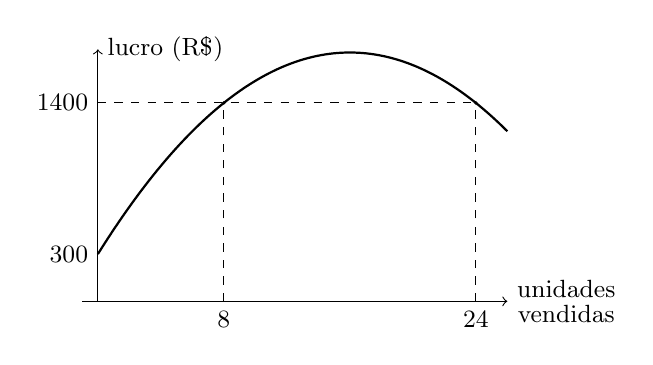
\begin{tikzpicture}[scale=0.2]
    % Eixos
    \draw[->] (-1,0) -- (26,0) node[right] {\small \shortstack{unidades \\ vendidas}};
    \draw[->] (0,0) -- (0,16) node[right] {\small lucro (R\$)};
    
    % Pontos de referência
    \draw[dashed] (8,0) -- (8,12.6);
    \draw[dashed] (24,0) -- (24,12.6);
    \draw[dashed] (0,12.6) -- (24,12.6);
    
    % Pontos e marcações
    \filldraw (8,12.6) circle (2pt);
    \filldraw (24,12.6) circle (2pt);
    \node[left] at (0,12.6) {\small 1400};
    \node[left] at (0,3) {\small 300};
    \node[below] at (8,0) {\small 8};
    \node[below] at (24,0) {\small 24};

    % Parábola
    \draw[domain=0:26, smooth, samples=100, thick]
        plot (\x, {-0.05*(\x-16)^2 + 15.8});
\end{tikzpicture}
\end{center}

\bigskip

\noindent Podemos concluir que o lucro máximo é de quanto?

\bigskip

% Define as alternativas
\newcommand{\alternativas}{%
    \begin{center}
        \begin{tabularx}{\textwidth}{XXXXX}
            (a) R\$ \(\n{1450,00}\). &
            (b) R\$ \(\n{1500,00}\). &
            (c) R\$ \(\n{1550,00}\). &
            (d) R\$ \(\n{1580,00}\). &
            (e) R\$ \(\n{1600,00}\).
        \end{tabularx}
    \end{center}
}

% Define a resposta correta
\newcommand{\resposta}{D}

% Lógica condicional para exibição
\ifdefstring{\atividade}{lista}{%
    \alternativas
    \vspace{0.5em}
    
    \noindent\textbf{Resposta:} letra \textbf{\resposta}.
}{%
    \ifdefstring{\modo}{objetivo}{%
        \alternativas
    }{%
        % modo = discursiva → não mostra alternativas
    }
}
\end{exercicioBanco}

